\section{How did you feel when your first child was born?}
During my pregnancy with Tim I realized how little I knew about the process of labor and delivery of a baby.
What could I expect? I had never talked at length with my mother about what her experiences of childbirth had been.
She had delivered 11 babies without one C-section.
All I knew from her experiences was that it was a routine process that brought a pregnancy to an end.
John and I went to classes and learned that indeed it is a unique and individual process for each woman.
It was also reassuring to know that I would not be alone during the process.
John agreed to be with me and our family doctor would attend as well.

Rather than go into more detail about the hours of labor that led up to the delivery let me say that relief and amazement are at least two feelings I experienced when blonde headed baby Tim appeared.
John had nearly fainted so I'm not sure where he was right away.
The doctor called Tim a banana head because his large blonde haired head had been molded as he pushed through the birth canal.
Another amazing part of this is the way fatigue fell away after I held the baby in my arms.
I'm sure it caught up with me later but the transition from a pregnant woman to a mother was astounding.
Here is this person who has been living quite intimately with me for most of the last year.
They had made their presence known before but we only now could begin to learn to know this person who had come into being as a result of our shared love.
I was awash in a sea of maternal love.
\begin{figure}
\centering
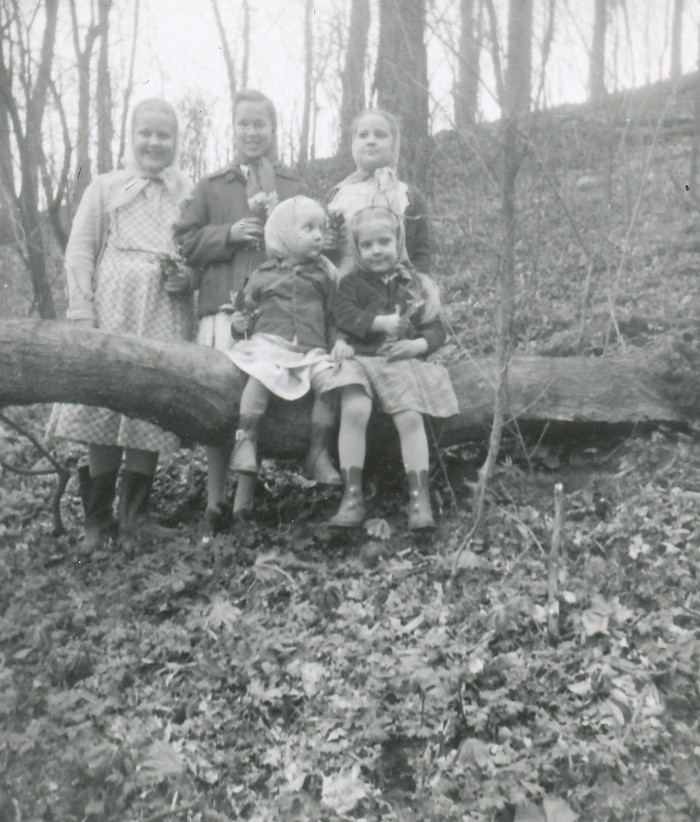
\includegraphics[width=0.9\textwidth]{our_family/5.jpg}
\caption{
Bringing Tim home from the hospital
}
\end{figure}

From Abby - This story both made me laugh out loud (the line about Dad fainting is hilarious and I also want to know more!) and tear up a little.
I am very excited to experience my own transition from pregnant woman to mother in just a few months.





